\documentclass[border=3mm]{standalone}

\usepackage{tikz}
\usetikzlibrary{arrows.meta,decorations.markings,calc}

\begin{document}
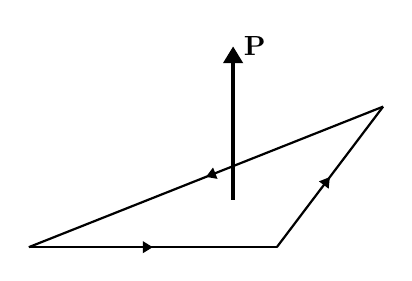
\begin{tikzpicture}[scale=0.75,decoration={markings,mark=at position 0.5 with {\arrow{Triangle[scale=0.75]}}}]
\draw[thick,postaction={decorate}] (-6.4,-1.6) coordinate (1)  -- (-2.2,-1.6);
\draw[thick,postaction={decorate}] (-2.2,-1.6) -- (-0.4,0.78) coordinate[pos=0.5](2);
\draw[thick,postaction={decorate}] (-0.4,0.78) -- (-6.4,-1.6);
\draw[very thick,-Triangle] (-2.94,-0.8) -- (-2.94,1.8) node[right] {$\mathbf{P}$};
\end{tikzpicture}
\end{document}